\documentclass[10pt,twocolumn,letterpaper]{article}

\usepackage{cvpr}
\usepackage{times}
\usepackage{epsfig}
\usepackage{graphicx}
\usepackage{amsmath}
\usepackage{amssymb}
\usepackage[utf8x]{inputenc}
\renewcommand{\refname}{Bibliografia}
\usepackage{listings}
\renewcommand{\lstlistingname}{}
\renewcommand{\figurename}{Figura}


\usepackage{url}

% Include other packages here, before hyperref.

% If you comment hyperref and then uncomment it, you should delete
% egpaper.aux before re-running latex.  (Or just hit 'q' on the first latex
% run, let it finish, and you should be clear).
%\usepackage[pagebackref=true,breaklinks=true,letterpaper=true,colorlinks,bookmarks=false]{hyperref}

\cvprfinalcopy % *** Uncomment this line for the final submission

\def\cvprPaperID{****} % *** Enter the CVPR Paper ID here
\def\httilde{\mbox{\tt\raisebox{-.5ex}{\symbol{126}}}}

% Pages are numbered in submission mode, and unnumbered in camera-ready
\ifcvprfinal\pagestyle{empty}\fi
\begin{document}

%%%%%%%%% TITLE
\title{Parallel Computing Mid-Term\\DES Decryption con C, Cuda \& OpenMP}

\maketitle
\thispagestyle{empty}

%%%%%%%%% ABSTRACT
\begin{abstract}
   L'obiettivo di questo progetto è quello di decifrare una password di otto caratteri avendo a disposizione il suo valore di hash, generato tramite algoritmo DES (Data Encryption Standard), e supponendo di conoscere il salt con cui è stata cifrata. In questa relazione verranno presentati e confrontati tre approcci diversi: uno sequenziale (in C) e due paralleli (con CUDA e OpenMP).
\end{abstract}

%%%%%%%%% BODY TEXT
\section{Introduzione}
In questo progetto vogliamo confrontare i tempi di esecuzione di un \textit{attacco con dizionario} all'algoritmo di cifratura DES utilizzando tre metodologie diverse.

Con l'espressione \textit{attacco con dizionario} si intende una tecnica di attacco alla sicurezza di un sistema, in cui si suppone di avere un dizionario di password in chiaro e fornendo una password cifrata, il programma dovrebbe scoprire se si trova nel dizionario, cifrando ad una ad una ogni parola per poi confrontare il risultato con l'hash della password.

\subsection{DES}
Il DES (Data Encryption Standard) è un algoritmo di cifratura basato su chiave simmetrica per cifrare e decifrare dati, risalente agli anni '70. Attualmente il DES è considerato insicuro perchè la chiave utilizzata per la cifratura è di soli 56 bit, il che lo rende facilmente vulnerabile agli attacchi. Negli ultimi anni tale algoritmo è stato sostituito dall'AES (Advanced Encryption Standard) \cite{DES}. 

\subsection{Descrizione del dataset}
Il dataset utilizzato per gli esperimenti è stato estratto da uno più grande contenente 10 milioni di password \cite{DATASET}. Con uno script Python sono state estratte solamente le password lunghe 8 caratteri e appartenenti al set [a-zA-z0-9]. Il dizionario finale contiene un milione e mezzo di password (file \textit{txt}, 13MB di dimensione).
\subsubsection{Scelta delle password da testare}
Per un confronto più accurato sui tempi di esecuzione, anziché selezionare le password casualmente sono state scelte dieci password uniformemente distribuite lungo il dizionario, riportate di seguito: \textit{'sirpizza', '3kingdom', 'tyleisha', 'marumari', 'giacomix', 'dbcookie', 'Yessssss', 'Mypaypa1', '6Melissa', '1Mazzola'}.

Per la valutazione dello speedup ottenuto con le due versioni parallele, invece, di queste dieci ne sono state selezionate tre (una all'inizio, \textit{'3kingdom'}, una a metà, \textit{'giacomix'}, e una alla fine, \textit{'6Melissa'}).

\subsection{Specifiche hardware}
Per questi esperimenti è stata utilizzata un'istanza \textit{EC2} di \textit{Amazon Web Services} con le seguenti specifiche:
\begin{itemize}
\item Istanza \textit{p2.xlarge} con accelerazione del calcolo
\item Processore a 2,3 GHz (base) e 2,7 GHz (turbo) Intel Xeon E5-2686 v4
\item GPU NVIDIA K80, ognuna con 2.496 core di elaborazione in parallelo
\item 90 GiB di memoria CPU e 12 GiB di memoria GPU
\end{itemize} 

\section{Implementazione}
Sono state eseguite tre implementazioni, una in maniera sequenziale in linguaggio C e due in maniera parallela rispettivamente con CUDA e OpenMP.

L'algoritmo DES non è stato implementato ma è stata usata la funzione \textit{crypt} per il C e \textit{crypt\_r} per OpenMP, entrambe definite nella libreria \textit{crypt} del C.

Per quanto riguarda CUDA, data l'assenza della libreria \textit{crypt}, è stata utilizzata un'implementazione open-source del DES specifica per la piattaforma \cite{DES-CUDA}.

Come \textit{salt}, per cifrare le password, è stata utilizzata una parola di due caratteri ("PC", Parallel Computing), in modo che \textit{crypt} e \textit{crypt\_r} facciano uso dell'algoritmo DES e non MD5, come indicato nel manuale della libreria GNU. \cite{SALT}

\subsection{Versione Sequenziale in C}
La versione sequenziale dell'algoritmo è piuttosto semplice. Dato in input il dizionario e la password cifrata da cercare, l'algoritmo scorre tutto il dizionario e ad ogni passo viene cifrata la parola corrente con DES. Se i due hash sono uguali, la password è stata trovata e il ciclo viene interrotto. Si itera fino alla fine del dizionario. 

Per misurare il tempo di esecuzione è stata utilizzata la funzione \textit{clock} della libreria standard del C \textit{time} che restituisce il tempo di CPU espresso in unità \textit{clock\_t} (colpi di clock). Per ottenere il risultato in secondi si divide per la costante CLOCKS\_PER\_SEC.
\newline

\begin{lstlisting}[basicstyle=\footnotesize, language=C, frame=single, caption={Esempio di ricerca sequenziale nel dizionario}, captionpos=b]
const char* password = "3kingdom";
char* enc = strdup(crypt(password, SALT));

while ((getline(&current, &len, dict)) != -1) {
  char* curr_enc = strdup(crypt(current, SALT));
  if (strcmp(enc, curr_enc) == 0) {
    // Password trovata!
    break;
  }
}
\end{lstlisting}

\subsection{Versione parallela con CUDA}
Data l'assenza di \textit{crypt} su piattaforma CUDA, è stata utilizzata una libreria esterna open-source per la cifratura DES: \textit{des-cuda} \cite{DES-CUDA}.
Questa espone un metodo \textit{full\_des\_encode\_block} che prende in input due valori di tipo \textit{uint64\_t} (interi a 64 bit, parola da cifrare e \textit{salt}) e restituisce a sua volta un \textit{uint64\_t} corrispondente alla cifratura DES della parola con il \textit{salt} fornito. Per adeguarsi, quindi, nella fase di preprocessamento tutte le parole del dizionario sono state convertite in interi a 64 bit. 

Dopo aver allocato e copiato la memoria necessaria da \textit{host} a \textit{device}, si effettua il lancio del \textit{kernel}, porzione di codice che viene eseguita in parallelo dai vari thread della GPU, con numero di \textit{blocchi} variabile e numero di \textit{grid} dipendente dalla dimensione del dizionario.
\newline

\begin{lstlisting}[basicstyle=\scriptsize, language=C, frame=single, caption={Esempio di lancio del kernel in CUDA},captionpos=b]
// Organizzazione blocchi e grid
dim3 blockDim(blockSize);
dim3 gridDim(DICTIONARY_SIZE/blockDim.x + 1);

// Lancio kernel
kernel<<<gridDim, blockDim>>>(device_dictionary, found);

// Copio risultato da device a host
CUDA_CHECK_RETURN(cudaMemcpy(psw_found, found, 
                  sizeof(uint64_t), 
                  cudaMemcpyDeviceToHost));
                  
if (*psw_found) {
  // Password trovata!
}
\end{lstlisting}

Il dizionario di parole viene salvato in memoria globale, in modo che sia condiviso tra tutti i thread, e viene passato come input al \textit{kernel}.

È stata utilizzata inoltre una variabile \textit{found} di tipo \textit{uint64\_t}, inizializzata a zero, che viene assegnata nel \textit{kernel} non appena un thread decifra correttamente la password. In questo modo, terminata l'esecuzione del \textit{kernel}, viene copiata la porzione di memoria relativa a questa variabile da \textit{device} a \textit{host}, ed è quindi possibile sapere se la password è stata decifrata correttamente.

In questo caso non è stato necessario chiamare il metodo \textit{cudaDeviceSynchronize()} dopo il lancio del kernel, solitamente utilizzato per attendere la terminazione di tutti i task della GPU, poichè la successiva operazione di copia di memoria (\textit{cudaMemcpy} di tipo \textit{cudaMemcpyDeviceToHost}) da sola garantisce che l'esecuzione avvenga in modo seriale, nonostante il lancio del kernel sia asincrono. 
In CUDA, infatti, tutte le operazioni che riguardano lo stesso \textit{stream} sono sincrone \cite{CUDA_SYNC}.

Se la password è stata trovata da un thread, come per la versione sequenziale, si misura il tempo di esecuzione utilizzando la funzione \textit{clock} della libreria standard \textit{time} del C. Per ottenere il risultato in secondi si divide per la costante CLOCKS\_PER\_SEC.\newline

Per quanto riguarda la memoria della GPU è stato scelto di salvare il \textit{salt} e la password cifrata da cercare nella \textit{device constant memory}, essendo entrambe informazioni costanti che non variano durante l'esecuzione del \textit{kernel} e che richiedono la sola lettura.

Ogni thread della GPU esegue il controllo su una sola parola, in base all'indice calcolato a partire dalle sue coordinate (\textit{blockIdx.x, blockDim.x} e \textit{threadIdx.x}).

Viene anche eseguito un ulteriore controllo per assicurarsi che l'indice del thread entri nei limiti della dimensioni del dizionario, in modo da evitare \textit{overflow} al contorno dell'ultimo blocco.\newline


\begin{lstlisting}[basicstyle=\scriptsize, language=C, frame=single, caption={Esempio di kernel in CUDA},captionpos=b]
__constant__ uint64_t salt;
__constant__ uint64_t encryptedPassword;

__global__ void kernel(uint64_t *dict, uint64_t *found) {
  int idx = blockIdx.x * blockDim.x + threadIdx.x;
  if (idx < DICTIONARY_SIZE) {
    uint64_t psw = dict[idx];
    uint64_t enc = full_des_encode_block(psw, salt);
    if (enc == encryptedPassword) {
      // Password trovata!
      *found = psw;
      return;
    }
  }
}
\end{lstlisting}

\subsection{Versione parallela con OpenMP}
Per quanto riguarda la versione parallela con OpenMP è stato scelto di utilizzare una classe, \textit{Decrypter}.

Il costruttore prende in ingresso il nome del file \textit{txt} relativo al dizionario e il \textit{salt} da utilizzare per la cifratura. Seguendo l'idioma RAII (\textit{Resource Acquisition Is Initialization}), il dizionario viene letto nel costruttore e ogni parola viene inserita in un vettore di stringhe, \textit{fullDictionary}, variabile privata della classe.

All'interno di \textit{Decrypter} è stato dichiarato anche un metodo, \textit{setPassword}, che salva in una variabile privata la password cifrata tramite la funzione \textit{crypt}. 

La classe espone inoltre un metodo \textit{decrypt}, che prende in ingresso il numero di thread da utilizzare nella direttiva di OpenMP \textit{\#pragma omp parallel num\_threads}, ed esegue l'algoritmo principale. Si scorre quindi l'intero vettore di password utilizzando la direttiva \textit{\#pragma omp for} e, all'interno del ciclo, la parola corrente viene cifrata tramite la funzione \textit{crypt\_r}, versione \textit{reentrant} di \textit{crypt}.

Poichè i cicli di OpenMP non possono essere interrotti, è stata utilizzata una variabile booleana di tipo \textit{volatile} (che garantisce la consistenza nella lettura del suo valore da parte di tutti i thread) per segnalare a tutti gli altri thread che la password è stata trovata, in modo che ciclino a vuoto senza eseguire alcuna istruzione finchè non terminano.

Il tempo di esecuzione è stato misurato utilizzando il metodo \textit{now()} della classe \textit{steady\_clock} della libreria \textit{std::chrono}.

\begin{lstlisting}[basicstyle=\scriptsize, language=C++, frame=single, caption={Esempio di ricerca in parallelo con OpenMP},captionpos=b]
double Decrypter::decrypt(int threads) {

  volatile bool found = false;
  auto start = chrono::steady_clock::now();

#pragma omp parallel num_threads(threads)
    {
  struct crypt_data data;
  data.initialized = 0;

#pragma omp for
  for (int i = 0; i < dict.size(); i++) {
    if (found) continue;
    char *current = crypt_r(dict[i], salt, &data);
    if (strcmp(current, encrypted) == 0) {
       // Password trovata!
       found = true;
    }
  }
    }

  if (found) {
    auto end = chrono::steady_clock::now();
    std::chrono::duration<double> s = end - start;
    return s.count();
  } else {
    return 0;
  }
}
\end{lstlisting}

\section{Esperimenti \& Risultati}
Per ogni esperimento sono state eseguite cinque iterazioni in modo da ottenere un misura più accurata dei risultati. Tutti i grafici presentati di seguito sono stati generati con uno script Python utilizzando la libreria \textit{matplotlib}.

L'accuratezza dei risultati ottenuti è stata valutata tramite la metrica dello \textit{speedup} (S), definito come il rapporto tra il tempo di esecuzione sequenziale ($t_s$) e il tempo di esecuzione parallelo ($t_p$): $S = \frac{t_s}{t_p}$.

\subsection{Valutazione dello Speedup con CUDA}
Date tre parole posizionate rispettivamente una all'inizio (\textit{"3kingdom"}), una in mezzo (\textit{"giacomix"}) e una alla fine (\textit{"6Melissa"}) del dizionario, è stato misurato lo \textit{speedup} al variare del numero di thread per blocco.

In particolare sono stati usati 8, 16, 32, 64, 128, 256, 512 thread per blocco (\textit{block\_size}), mentre il numero di blocchi per ogni \textit{grid} è data dalla formula $\frac{dictionary\_size}{block\_size}+1$, dove $dictionary\_size$ è il numero di parole presenti nel dizionario.
\begin{figure}[h]
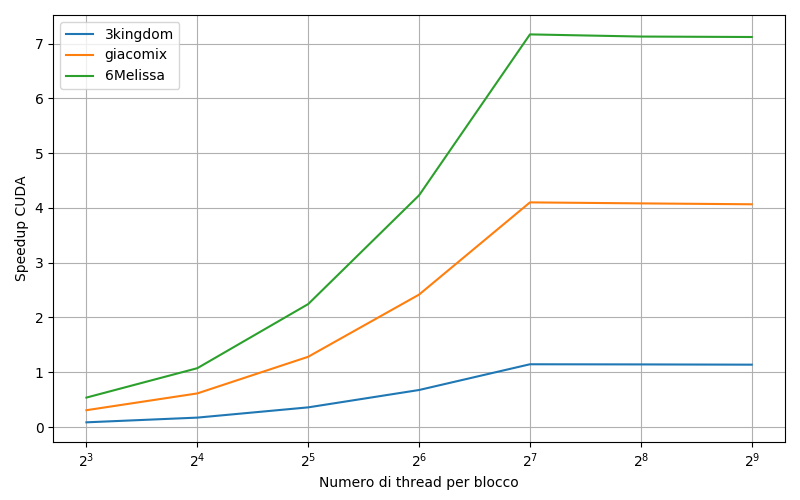
\includegraphics[width=\linewidth]{Plots/tempi_cuda.png}
\caption{Speedup in CUDA}
\label{fig:tempi_cuda}
\end{figure}

Come si può vedere dalla figura \ref{fig:tempi_cuda} lo \textit{speedup} maggiore si ottiene con le parole posizionate in fondo al dizionario e il suo valore cresce all'aumentare del numero di thread per blocco, stabilizzandosi e rimanendo costante dopo 128 thread per blocco. 

Come era verosimile aspettarsi, soltanto per parole all'inizio del dizionario risulta più efficiente la versione sequenziale ($speedup \le 1$) soprattutto con numero limitato di thread per blocco.

\subsection{Valutazione dello Speedup con OpenMP}
Date tre parole posizionate rispettivamente una all'inizio (\textit{"3kingdom"}), una in mezzo (\textit{"giacomix"}) e una alla fine (\textit{"6Melissa"}) del dizionario, è stato misurato lo \textit{speedup} al variare del numero di thread di OpenMP. In particolare sono stati usati 8, 16, 32, 64, 128, 256, 512, 1024, 2048, 4096 thread.

\begin{figure}[h]
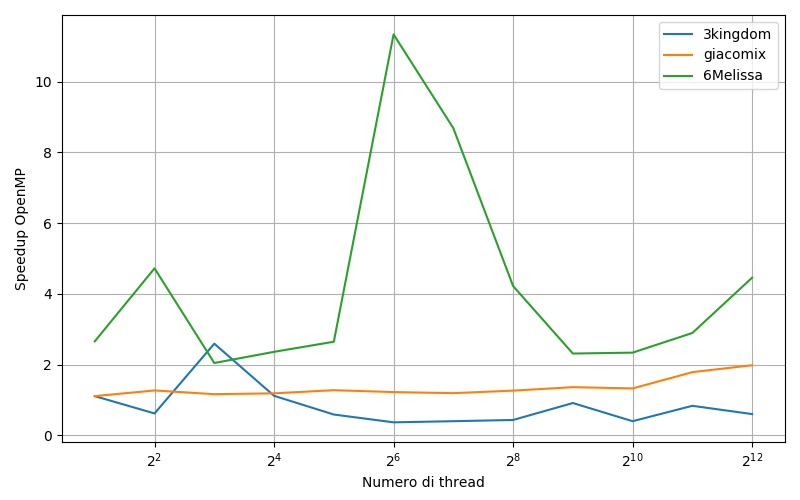
\includegraphics[width=\linewidth]{Plots/tempi_openmp.png}
\caption{Speedup in OpenMP}
\label{fig:tempi_openmp}
\end{figure}

Come si può vedere dalla figura 	\ref{fig:tempi_openmp}, in generale lo \textit{speedup} maggiore si ottiene con le parole posizionate in fondo al dizionario; in particolare con la parola \textit{"6Melissa"} presa in esame è possibile ottenere uno \textit{speedup} maggiore di 11 con 64 thread. Questo si tratta però chiaramente di un caso fortunato e totalmente dipendente dalla posizione che assume la parola nella divisione automatica in \textit{chunk} da parte di OpenMP.

Per le parole all'inizio del dizionario, come ad esempio \textit{"3kingdom"}, la parallelizzazione con OpenMP risulta invece poco efficiente anche all'aumentare del numero di thread in confronto alla versione sequenziale (infatti $speedup \le 1$ quasi ovunque). Questo risultato può essere attribuito all'elevato \textit{overhead} introdotto dalla gestione dei thread.
\subsection{Confronto sui tempi di esecuzione}
Per un'ulteriore valutazione sono state quindi scelte dieci parole uniformemente distribuite lungo il dizionario, in modo da poter confrontare direttamente i tre approcci diversi (C, CUDA e OpenMP) in alcuni casi particolari.

In CUDA è stato scelto il caso con 128 thread per blocco, mentre per OpenMP è stato scelto il caso con 32 thread.

\begin{figure}[h]
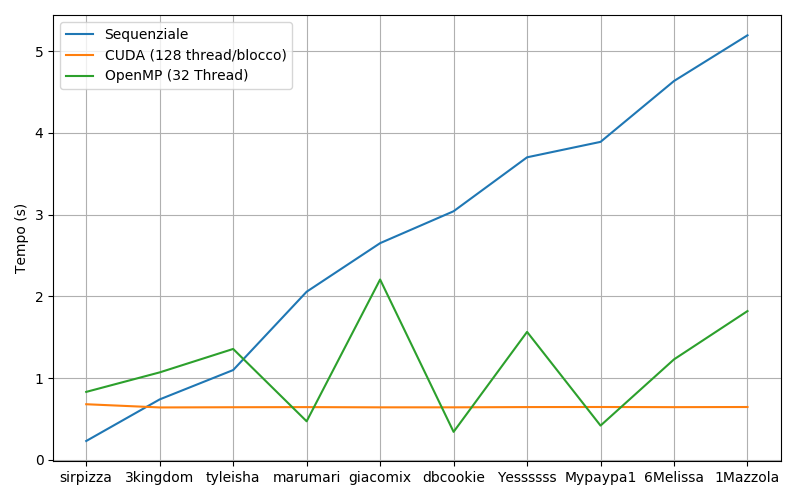
\includegraphics[width=\linewidth]{Plots/tempi.png}
\caption{Confronto tempi di esecuzione}
\label{fig:tempi}
\end{figure}

Come si può chiaramente notare dalla figura \ref{fig:tempi}, da un certo punto in poi del dizionario ($\approx25\%$) entrambi gli approcci paralleli risultano sempre più efficienti rispetto all'approccio sequenziale.

Come prevedibile, il tempo richiesto per la versione sequenziale aumenta linearmente con lo scorrere della posizione delle parole verso il fondo del dizionario. 

In CUDA, indipendentemente dalla posizione nel dizionario della parola scelta, il tempo di esecuzione rimane costante ($\approx0.7$ secondi).

Con OpenMP, invece, il tempo di esecuzione presenta delle oscillazioni, riuscendo in alcuni casi particolari ad ottenere tempi di esecuzioni inferiori rispetto a CUDA. Come detto prima, questi casi sono del tutto fortuiti in quanto dipendono dalla posizione della parola nel \textit{chunk} di OpenMP.

\section{Conclusione}
Come era possibile aspettarsi il migliore approccio per un \textit{attacco con dizionario} risulta essere quello parallelo.

Il problema principale delle versioni parallele potrebbe essere quindi quello della ricerca del numero ottimale dei thread affinché si ottenga lo \textit{speedup} migliore.

Da una parte OpenMP risulta sicuramente più facile da implementare rispetto a CUDA, in quanto la parallelizzazione avviene in maniera del tutto automatica (anche se con poca flessibilità sulla scelta del modo in cui vengono divisi i dati).

Dall'altra parte l'utilizzo di CUDA risulta più macchinoso, richiede molte più attenzioni e soprattutto risorse (una o più GPU di calcolo), ma offre un tempo di esecuzione sempre costante e fino a sette volte più performante rispetto alla versione sequenziale.

{
\bibliographystyle{unsrt}
\bibliography{bibliografia.bib}
}


\end{document}
